\chapter{Segmentation}

We discuss how we use the Frangi as a prefilter and discuss several different segmentation strategies, and describe our "strawman" which is the ISODATA threshold. First, we define some quantitative measures of success for segmentations


\subsection{Binary Classifications and the confusion matrix}

We wish to come up wish a means of gauging the success of our segmentations and will adopt a binary classification model to do so.
We end up with a boolean matrix the size of the image, and compare it to the ground truth, the trace, and then compare them to get the number of true positives, true negatives, false positives, and false negatives. We demonstrate these visually with a confusion matrix, as in cref{fig:sample-confusion}.
\begin{figure}
  \centering
  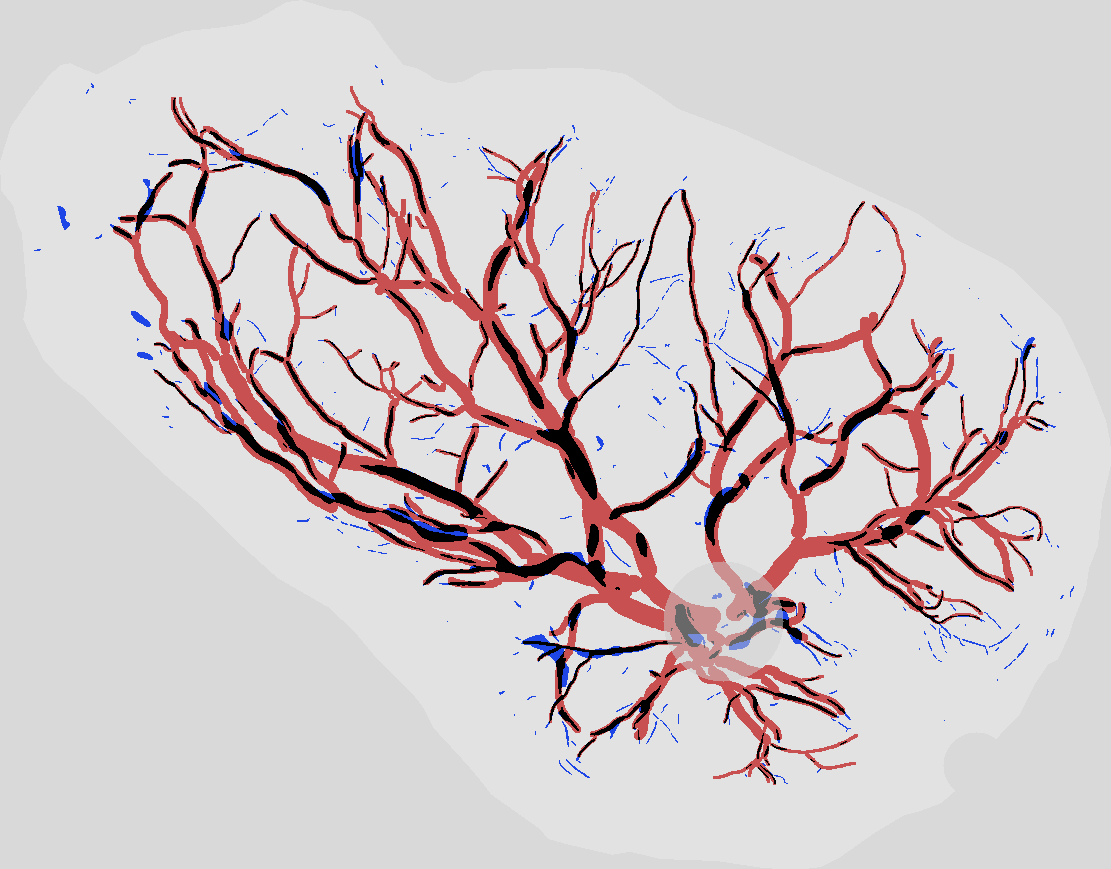
\includegraphics[width=\textwidth]{sample_confusion}
  \caption{Sample confusion matrix}
  \label{fig:sample-confusion}
  
\end{figure}

Although there are many measures to gauge the success of binary classification, we will focus on two that we find particularly illustrative. The first is precision, given by

\begin{equation}
\label{eq:precision}
\textrm{precision} \;=\; \frac{TP}{TP+FP}
\end{equation}

and the second is the Matthews Correlation Constant (MCC), given by

\begin{equation} \label{eq:MCC}
MCC = \frac{TP\times TN - FP \times FN}{\sqrt{ (TP + FP)(TP+FN)(TN+FP)(TN+FN)}}
\end{equation}

where precision is a ratio between 0 \% and 100\% and the MCC is a measure between -1 and 1. Precision (or positive predictive power) is of course a ratio between how many labels we got correct over all pixels we labeled as positive. This is a useful score for us--if we are using Frangi as a prefiltering for a more robust technique, we would not want to provide any wrong information or seeds to that algorithm. Precision therefore does an okay job of representing that scenario: we are not penalized for what we do not label as true, as long as our reports of true are correct.

Of course, we cannot rely on precision as our sole quantiative factor alone--we could simply return everything negative and recieve a perfect score of 100\% precision. Therefore we will gauge that measure with that of the MCC \cite{mcc-original-paper}. The main advantage of the MCC is that is well balanced no matter what the size of the two classes are, and will only be high if the approximation scores well against both labels. A score of $1.0$ means the approximation is 100\% correct, a score of $-1.0$ means that everything is completely incorrect, and a score of $0$ means that the test performs only as well as random guessing. In our analysis, we will consider both the MCC and precision of a particular segmentation simultaneously. We would like an MCC score as high as possible, but will contextually settle for a lower score as long as the approximation is still textit{precise}.

One final point about these measures is that we have decided to report their scores only within the placental plate, rather than the entire rectangular image. Since the area outside of plate is masked from consideration, those points will be true negatives no matter what, and we don't want this artificial padding to influence our score. That being said, we do currently concede one part right now: we will also mask an area around the umbilical cord insertion point, as the large amount of noise here will mean that our scores are artificially low. We would like to remove these areas, but for now we will simply not score them. 

\section{Postprocessing Techniques}
We display several four relatively immediate postprocessing techniques on the multiscale Frangi output to obtain an actual PCSVN extraction. Again we stress that the Frangi filter itself does not produce a segmentation, but instead could be used as a preprocessing step. In fact, Frangi in his original paper \cite{frangi-paper} refrained from any explicit analysis of the Frangi score apart from taking the maximum across all scales, as in \cref{frangi-vesselness-max}. Still, we wish to demonstrate some several immediate methods of postprocessing these samples in order to illustrate the usefulness of this optimized Frangi filter. 

Unfortunately, even with our ``rescaled'' Frangi filter, this $\alpha$ cannot be picked without regard for the particular image domain. Equally problematic, we cannot guarantee that the Frangi filter will decay as our scale exceeds the the bounds where structure is expected to be found. Ideally we could create a filter that would do that.

\subsection{Method A: Fixed Threshold}

In the fixed threshold method, we say that a pixel $(x,y)$ of the image corresponds to a vessel if
$V_{\max} >  \alpha$. This $\alpha$, as noted above, is unfortunately highly dependent on the image domain, and this merging method will tend to happily allow noise generated from scales that are too large or too small. \vtodo{PUT A FIGURE HERE OF BIG BLOTCHES WHEN THE SCALE IS TOO LARGE}. Another issue with this is the individual scales of the Frangi filter in the extreme cases are not known to scale--although Lindeberg introduced a normalization factor based on the scale to apply to the derivatives, we do not know of an optimal factor to use.


\subsection{Method B: Percentile Based Merging}

The idea behind percentile-based merging is beneficial for large multiscale methods. At each scale, we would like to assume that there is \textit{some} curvilinear content that could be identified. With that in mind, we could simply accept from each scales scores in a very high percentile. We chose for our demonstration a fairly large percentile, $95$, and furthermore boster this by requiring that any selected pixels be in the 95th percentile of nonzero and unmasked pixels--otherwise the average is artificially low due to the large background and pixels with zero Frangi score. The use of percentiles removes dependence of picking a particular threshold on the problem, while allowing the most prominent features to emerge at each scale, but of course it unfortunately treats all scales equally, so the success of the multiscale approach here is very dependent on choice of $\sigma_{\min}$ and $\sigma_{\max}$.

\subsection{Method C: Scale-Based Random Walker}

We observed that areas where Frangi scores are zero in well-behaved samples seem to neatly outline prominent vascular features. Following this idea, we employed a random walker segmentation \cite{Grady-Random-Walks} (which is implemented by \texttt{scikit-image}). Random walk segmentation comes about by solving a diffusion problem over a discrete array (in this case, the Frangi vesselness score itself) given starting markers. At each scale, we positively labeled pixels whose Frangi score was very high ($V_\sigma(x_0,y_0) > .4$), and negatively labeled pixels whose score was $0$ (i.e. where the leading principal eigenvalue was positive). The result of this technique is demonstrated in \cref{rw_demo-scalewise} and the result (along with the original sample for comparison) is shown in \cref{fig:rw-demo-merged}.
In \cref{rw-demo-scalewise}, the first column is the Frangi vesselness score at that scale, where black is a score of 0, to emphasize the difference between a score of zero and even a very small positive score, which appear in blue. The middle score are markers passed to the random walker--blue are seeds labelled with a ``1'' (where the Frangi vesselness score is 0), green is labeled ``2'' (where V > .4), and purple represents unknowns that will either assigned either label. In the last column, the result of the random walker is given--areas that have been added to the label ``2'' are shown in yellow. Although the result of random walker segmentation is technically a binary matrix, we still show the original seeds of label 2 in green for easier comparison. Similarly, the purple in the right column has actually been labeled ``1'' for non-vascular, but is left in its original color to emphasize what was assigned background. In \cref{fig:rw-demo-merged} we show the original image and the result of merging all positively marked pixels at each scale. Black means the pixel was unmatched, while increasing colors of blue (larger scales) to white (smaller scales) indicate the smallest scale from which a pixel was marked after the random walker technique. \vtodo{Do I need to over this in math methods section?} Though we shall set up the multiscale method slightly differently in \cref{ch:results-analysis}, we used a Frangi anisotropy coefficient of $\beta=0.35$ , and 12 scales logarithmically spaced from $\sigma_1 = 2^{-1.5} $ to $\sigma_12 = 2^{3.5}$ to generate these figures. There is a coefficient (also called $\beta$) which serves as a diffusion penalization coefficient (larger values making diffusion over the image less likely). We used \texttt{scikit-image}'s default value of 130. 

\begin{figure}[p] \centering
  \subfloat{
    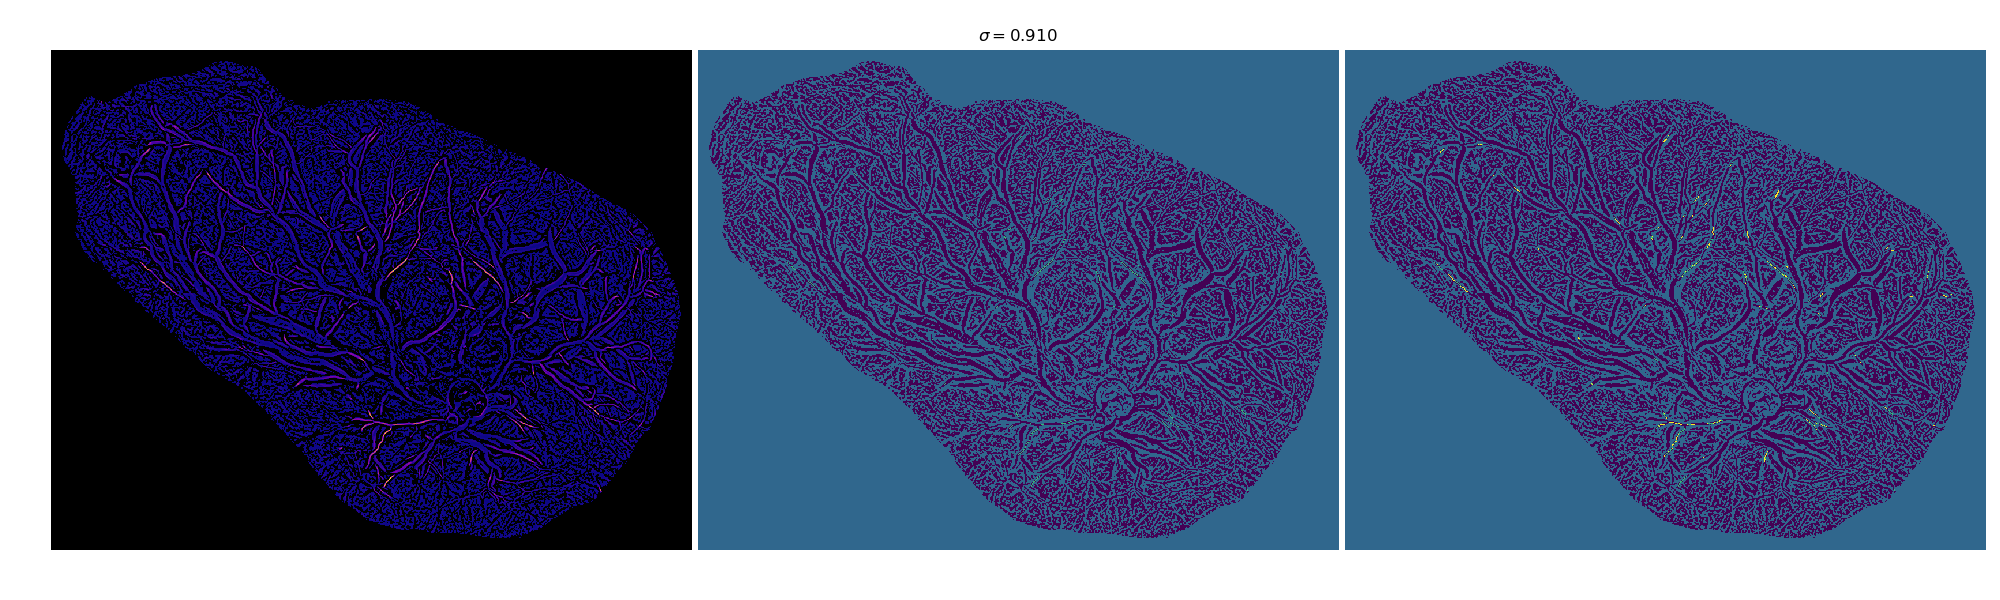
\includegraphics[width=\textwidth]{rw_demo_scale_03}
  }\\[-0.5cm]
  \subfloat{
    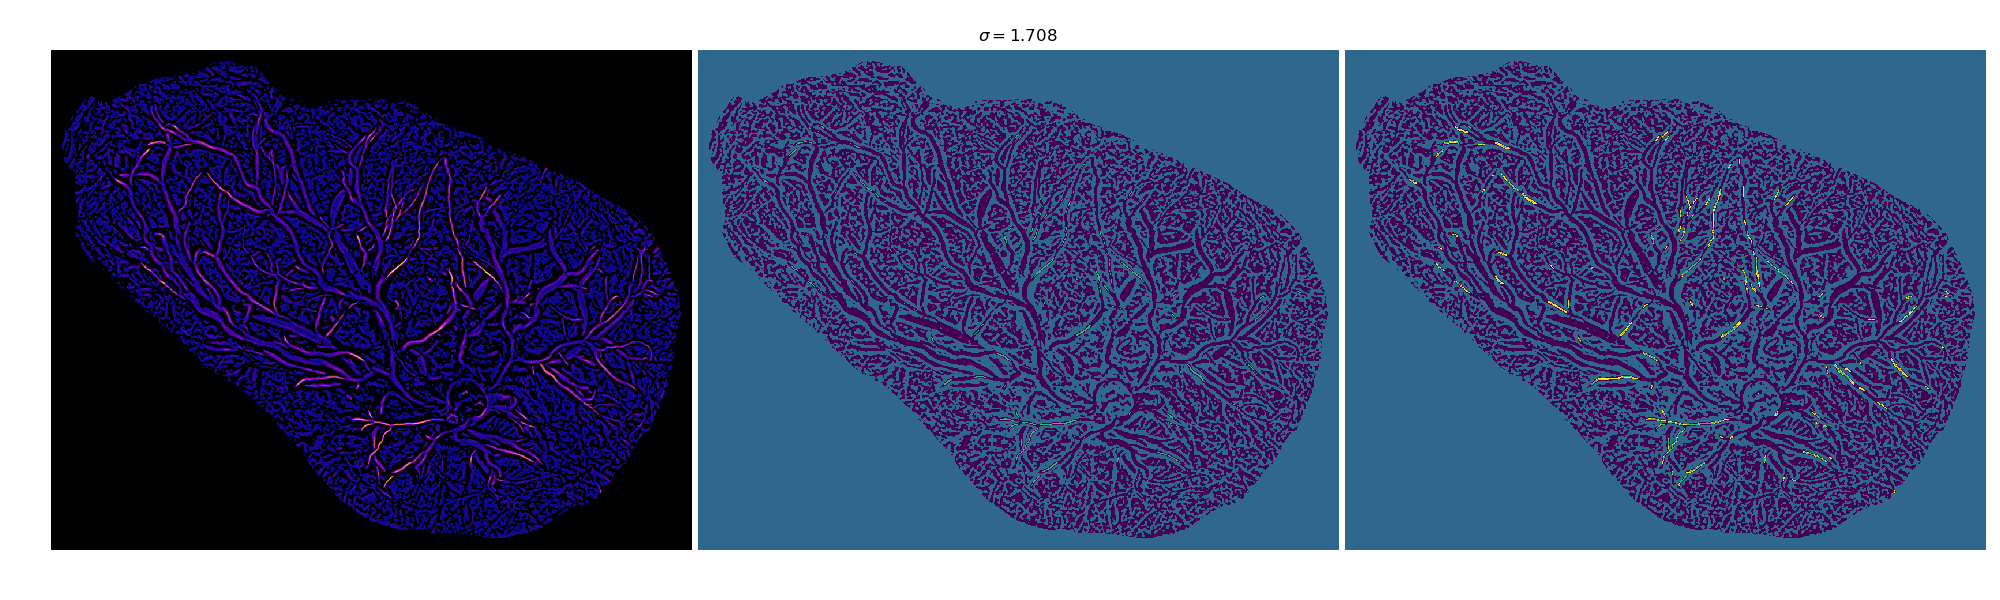
\includegraphics[width=\textwidth]{rw_demo_scale_05}
  }\\[-0.5cm]
  \subfloat{
    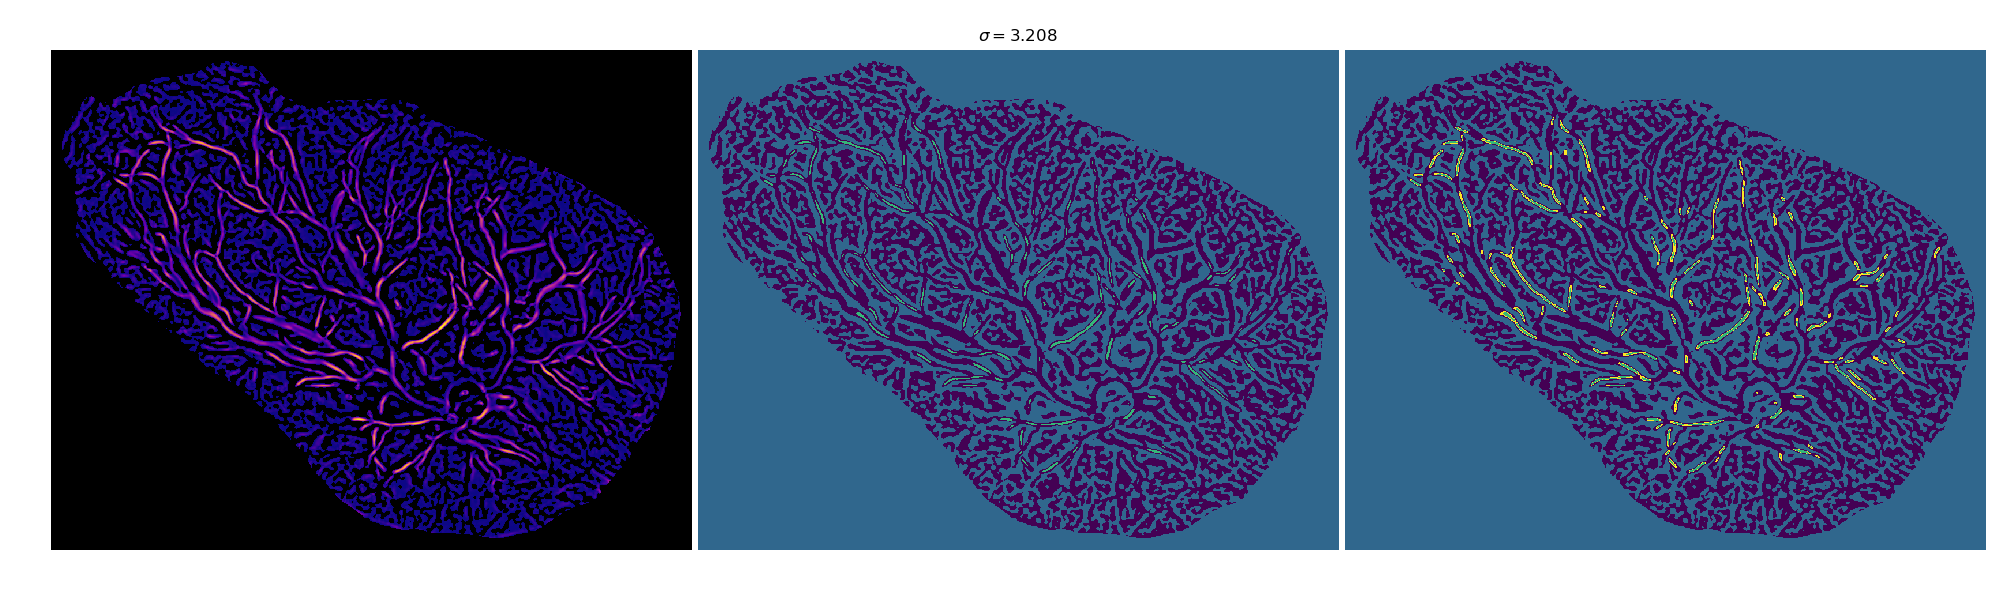
\includegraphics[width=\textwidth]{rw_demo_scale_07}
  }\\[-0.5cm]
  \subfloat{
    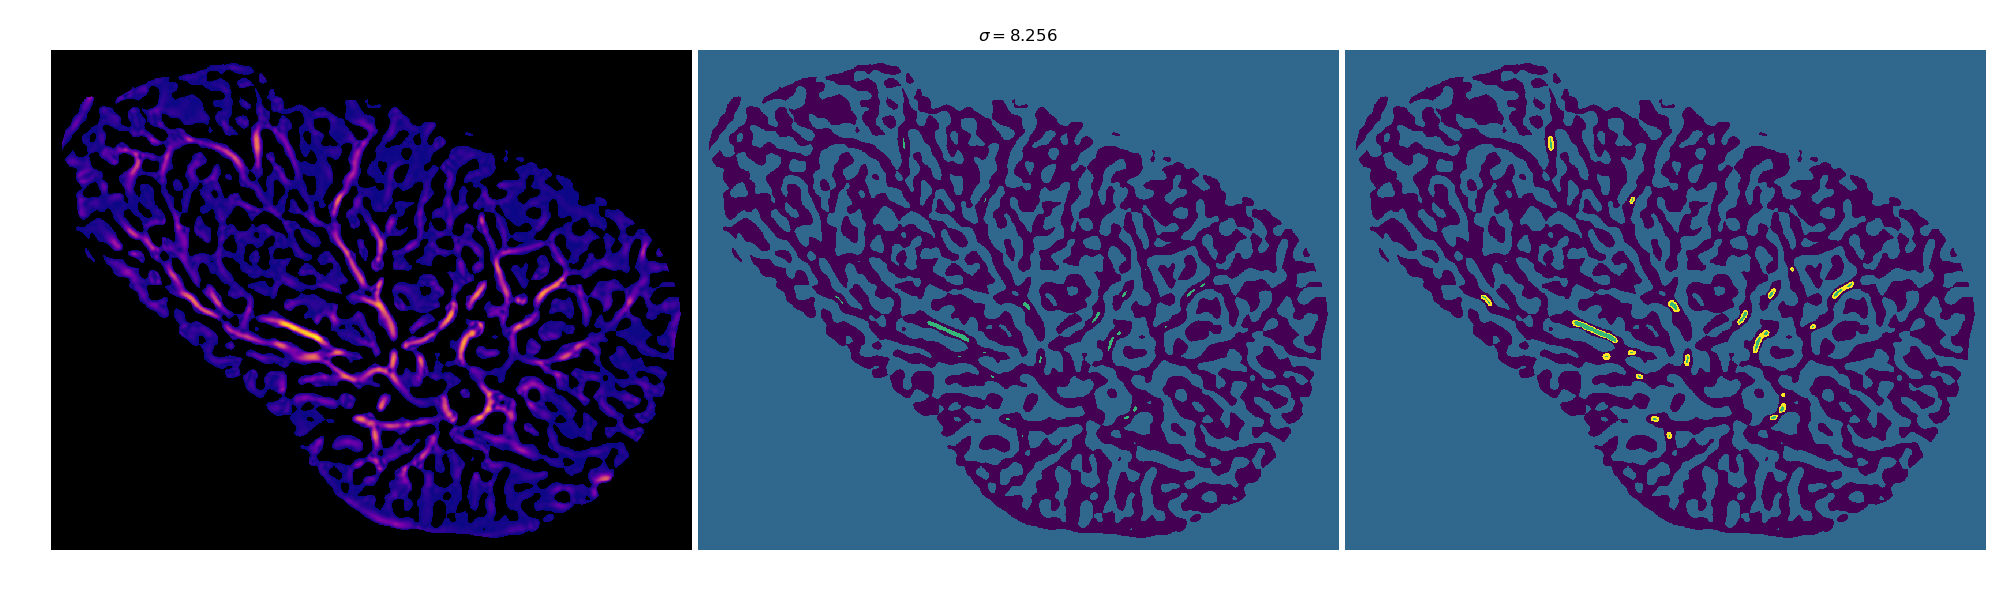
\includegraphics[width=\textwidth]{rw_demo_scale_10}
  }
  \caption{Scale-wise random walker segmentation (select scales)}
  \label{fig:rw-demo-scalewise}
\end{figure}


\begin{figure} \centering
  \subfloat{
    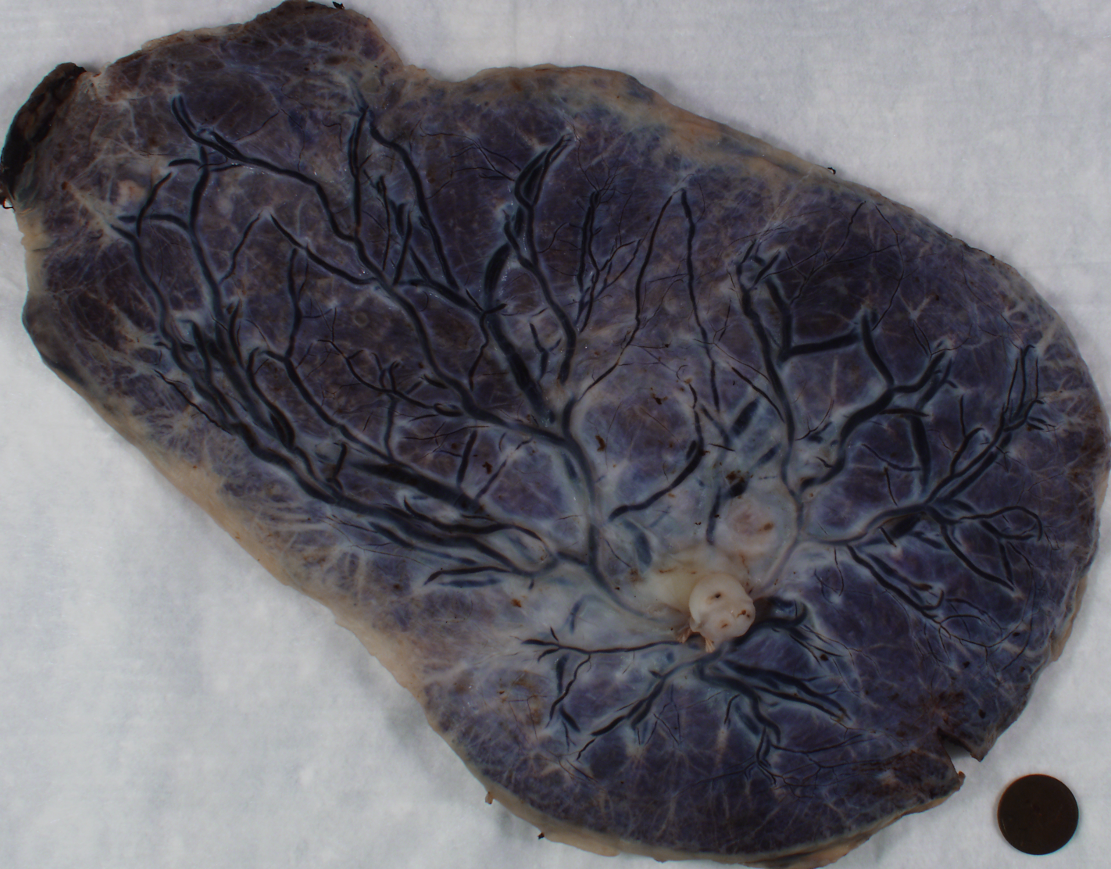
\includegraphics[height=0.3\textheight]{rw_demo_base}
  }\\
  \subfloat{
    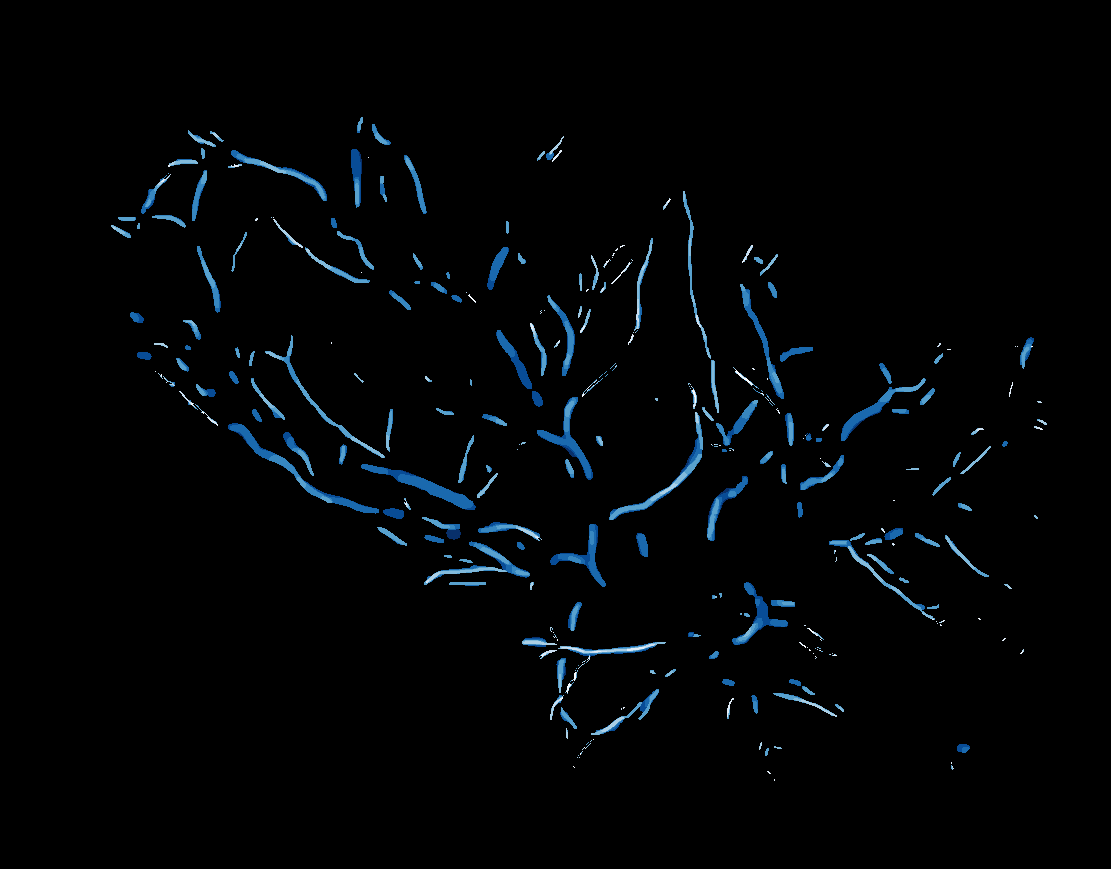
\includegraphics[height=0.3\textheight]{rw_demo_labels}
  }
  \caption{Random walker segmentation (result and sample)}
  \label{fig:rw-demo-merged}
\end{figure}

\subsection{Method D: Scale Based Sieving}

Our final approach seeks to include not only pixels at each scale that pass a high threshold, but also adjacent pixels at that scale that pass a lower threshold. We proceed as follows. At each scale, take a low threshold, then label each connected region. Then, iterate through each labeled region and add to the final approximation any labeled region that contains a pixel that passes a higher threshold.